\documentclass[a4paper,12pt,oneside]{article}
\usepackage{amsmath}
%\usepackage{mathtools}
\usepackage{caption}
\usepackage{mathptmx}
\usepackage{graphicx}
\usepackage[margin=1.0in]{geometry}
\usepackage{float}
\usepackage{setspace}
\usepackage{chngcntr}
\usepackage{fancyhdr}
\pagestyle{fancy}
\fancyhf{}
\rfoot{\thepage}
%\renewcommand{\headrulewidth}{0.0pt}
%\renewcommand{\footrulewidth}{0.0pt}

\begin{document}
\thispagestyle{empty}
%\pagenumbering{gobble}
\begin{center}

\large{\textbf{Wi-Vi Technology - See Through Walls}
\setlength{\baselineskip}{1.5\baselineskip}}
\\

\vspace{5mm}
\textbf{SEMINAR REPORT}
\\
\vspace{3mm}
Submitted in the partial fulfilment of the award of the degree
of
\vspace{3mm}
\\
\textbf{Bachelor of Technology}
\\
\vspace{3mm}
in
\\
\vspace{3mm}
\textbf{Computer Science and Engineering}
\\
\vspace{3mm}
of
\\
\vspace{3mm}
\textbf{APJ Abdul Kalam Technological University}
\\
\vspace{3mm}
by
\\
\vspace{3mm}
\textbf{Manimaran N}
\\
\vspace{5mm}
\begin{figure}[H]
	\centering
	
\includegraphics{ceclogo.png}
\end{figure}
\vspace{25mm}
\textbf{November, 2018}
\vspace{8mm}
\\
\vspace{2mm}
Department of Computer Engineering
\\
\vspace{2mm}
College of Engineering, Chengannur, Kerala -689121
\\
\vspace{2mm}
Phone: (0479) 2454125, 2451424; Fax: (0479) 2451424
\\


\end{center}

\newpage
\thispagestyle{empty}
\begin{center}
\setlength{\baselineskip}{1.5\baselineskip}
{\large\textbf{COLLEGE OF ENGINEERING, CHENGANNUR}}
\\
{\large\textbf{KERALA}}
\\
\begin{figure}[H]
\centering

\includegraphics{ceclogo.png}
\end{figure}
\setlength{\baselineskip}{1.5\baselineskip}
\textbf{Department of Computer Science and Engineering}
\\
\textbf{CERTIFICATE}
\\
This is to certify that the seminar entitled
\\
\textbf{Wi-Vi Technology - See Through Walls}
\\
Submitted by
\\
\textbf{Manimaran N}
\\
is a bonafide record of the work done by him.
\end{center}
\vspace{8mm}
\vspace{14ex}
%\textbf{Mrs.Shiny}
\hspace{55ex}
%\textbf{Dr. Smitha Dharan}
\\
\vspace{2ex}
\hspace{0ex}
\textbf{
Co-ordinator}
\hspace{45ex}
\textbf{
Head of The Department}
\newpage
\pagenumbering{roman}


\renewcommand{\headrulewidth}{0.0pt}
\renewcommand{\footrulewidth}{0.0pt}



\begin{center}
\large{\textbf{ACKNOWLEDGEMENT}}
\end{center}
\vspace{6ex}
\setlength{\baselineskip}{1.5\baselineskip}

\paragraph{}
I am greatly indebted to God Almighty for being the guiding light throughout with his
abundant grace and blessings that strengthened me to do this endeavour with confidence.
\paragraph{}
I express my heartfelt gratitude towards \textbf{Dr. Jacob Thomas V.}, Principal, College
of Engineering Chengannur for extending all the facilities required for doing my seminar.
I would also like to thank \textbf{Dr. Smitha Dharan}, Head, Department of Computer
Engineering, for providing constant support and encouragement.
\paragraph{}
Now I extend my sincere thanks to my seminar co-ordinators \textbf{Mrs.Shiny Balakrishnan}, Associate
Professor in Computer Engineering and \textbf{Ms. Angel Thomas} , Assistant
Professor in Computer Engineering for guiding me in my work and providing timely
advices and valuable suggestions.
\paragraph{}
Last but not the least, I extend my heartfelt gratitude to my parents and friends for
their support and assistance.	

\pagenumbering{gobble}
\newpage

\begin{center}
\large{\textbf{ABSTRACT}}
\end{center}
\vspace{6ex}
\paragraph{}

Wi-Vi, is based on a concept similar to radar and sonar imaging, but rather than using
high-power signals, this tech uses reflected Wi-Fi signals to track the movement of people
behind walls and closed doors. When a Wi-Fi signal is transmitted at a wall, a portion of that
signal penetrates through and reflects off any humans that happen to be moving around in the
other room. Since only a tiny fraction of the signal passes through the wall, with the rest being
reflected, the researchers had to devise a technology that could cancel out the arbitrary
reflections, and keep only those reflecting from moving human bodies. under this technology
communication is possible by combination of gestures and by messaging without even using any
transmitter. In this paper two innovations are being introduced: (1) Use of MIMO interfacing to
nullify the effect of static object and focusing the receiver on a moving target (2) motion of a
human body is treated as an antenna and resulting RF beam is tracked. Not much research has
been done on this technology but Wi-Vi could be built into a smart phone or a special handheld
device and used in search-and-rescue missions and law enforcement.
 To exemplify, someone walking outdoors at night who thought they were being followed
might use it to detect a person behind a fence or around a corner. The key benefits of Wi-Vi over
current ways of seeing through walls, such as radar and sonar, are cost, power and size. At the
heart of the technology is its encoding scheme, which can be implemented in silicon. WiVi could
be built into a cell phone soon, and for not much more than the cost of a regular Wi-Fi module.
Bringing wall-penetrating vision to handheld devices could open up a lot more uses for it.
Current radar-based systems used in the U.S. military are so big they need to be transported on
trucks. Even the Army might need a more portable tool for seeing through walls in certain
settings. Because of its low resolution, Wi-Vi could actually enhance people's privacy rather than
erode it in some cases.

\setlength{\baselineskip}{1.0\baselineskip}
\newpage
\begin{center}
\tableofcontents
\end{center}
\newpage
\thispagestyle{plain}
\begin{center}
\vspace{5mm}
\listoffigures
\vspace{5mm}
2.1 ULTRA WIDE BAND SYSTEM……………………………………………..12
\\
\vspace{4mm}
2.2 WISEE……………………………………………………………………13
\\
\vspace{4mm}
2.3 GESTURES……………………………………………………………….14
\\
\vspace{4mm}
2.2 APPLICATIN OF WISEE…………………………………………………...15
\\
\vspace{4mm}
3.3 ANTENNA ARRAY………………………………………………………...18
\\
\vspace{4mm}
4.1 EXPERIMENTAL SET UP…………………………………………………...19
\\
\vspace{4mm}
4.2 TRACKING SINGLE HUMAN……………………………………………....20
\\
\vspace{4mm}
4.3 ELIMINATING FLASH EFFECT……………………………………………...20
\\
\vspace{4mm}
5.0 TRACKING TECHNIQUES…………………………………………………27
\\
\vspace{4mm}
5.1 GESTURE TECHNIQUES…………………………………………………..22

\end{center}





\newpage
\rfoot{\thepage}

\lhead{\textit{Wi-Vi Technology - See Through Walls}}

\lfoot{\textit{College of Engineering, Chengannur}}

\rfoot{\thepage}

\renewcommand{\headrulewidth}{0.0pt}
\renewcommand{\footrulewidth}{0.0pt}




\renewcommand{\headrulewidth}{0.0pt}
\renewcommand{\footrulewidth}{0.0pt}



\section{INTRODUCTION}
\pagenumbering{arabic}
\paragraph{}
The use of WI-FI signal is not only as an information carrier; these WIFI signals can be used to track the moving object behind the wall or can say in a close room. This idea can be used to minimize the causalities in standoff and hostage condition, emergency responder can be used to see through wall, rubber or collapsed structure.
\paragraph{}
To recognize moving object through wall the WIFI signal transmitted in the direction of
wall, this results in two problem (I) Flash effect, (II) magnitude of signal reduced by three to five
times after traversing the wall. To solve these problems systems are developed and experiments
performed on those systems to achieve the desired results. The radar community developed a
system named Ultra-Wideband. This system detects human behind the wall and shows moving
blobs in output screen. To overcome the drawbacks of this system two new system were
developed named WI-VI and WISEE. These both systems use WI-FI signal to recognize the
moving object behind the wall. WISEE system works on the Doppler Sift principle, for the
human gesture it gives the different Doppler pattern according to the movement of any human.
But the problem with this system is, very small change in Doppler shift for the human gesture
which is very difficult to detect. On the other hand WI-VI system also use WI-FI signals to
recognize the moving object behind the wall, this system use the nulling technique to remove the
flash effect. This system not require large antenna array, it only need three small antenna MIMO
radio interface. Flash effect term refers to “The reflection from the entire stationary object
behind the wall rather than just wall”, which is much stronger than the reflection from the object
inside the closed room.


\newpage
\section{History}
\paragraph{}
Its research has been done prominently at MIT’s(Massachusetts Institute of Technology)
Computer Science and Intelligence Laboratory. By Dina Kitabi, a professor in MIT’s Department
of Electrical engineering and computer science, and her graduate student Fadel Adib.
\paragraph{}
In the 1930s, U.S. Navy researchers stumbled upon the concept of radar when they
noticed that a plane flying past a radio tower reflected radio waves. Scientists have now applied
that same principle to make the first device that tracks existing Wi-Fi signals to spy on people
through walls. Wi-Fi radio signals are found in 61 percent of homes in the U.S. and 25 percent
worldwide, so Karl Woodbridge and Kevin Chetty, researchers at University College London,
designed their detector to use these ubiquitous signals. When a radio wave reflects off a moving
object, its frequency changes a phenomenon called the Doppler effect. Their radar prototype
identifies frequency changes to detect moving objects. It's about the size of a suitcase and
contains a radio receiver composed of two antennas and a signal-processing unit. In tests, they
have used it to determine a person's location, speed and direction—even through a one-foot-thick
brick wall. Because the device itself doesn't emit any radio waves, it can't be detected.
\paragraph{}
Wi-Fi radar could have domestic applications ranging from spotting intruders to
unobtrusively monitoring children or the elderly. It could also have military uses: The U.K.
Ministry of defence has funded a study to determine whether it could be used to scan buildings
during urban warfare. With improvements, Woodbridge says, the device could become sensitive
enough to pick up on subtle motions the ribcage makes during breathing, which would allow the
radar to detect people who are standing or sitting still.









\subsection{Previous Technology}

\paragraph{}
This system is recently developed by the radar community to detect the moving object
behind the wall which give moving blobs as a result for the moving object behind the wall. This
system separates reflection from wall or other static object and the reflection from moving object
behind the wall based on their arrival time, so it must required to identify delays of even subnanoseconds.

\begin{figure}[H]
\centering
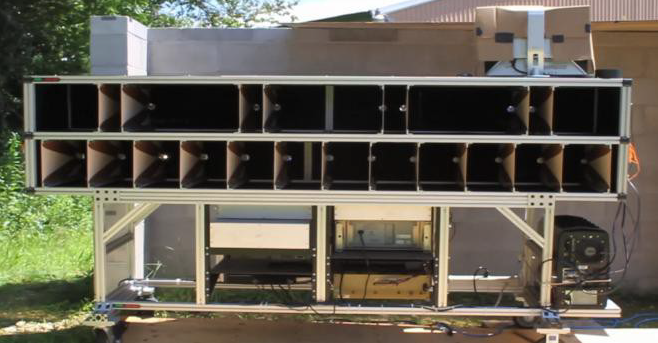
\includegraphics[height=10cm,width=14cm]{1.png}
\counterwithin{figure}{section}
%\counterwithout{figure}{chapter}
\end{figure}

\paragraph{}
The system shown above in Fig requires 2GHz of bandwidth, a very large power
source, and around 8-foot long antenna array and most important parameter is that the large
power in such a wide spectrum is infeasible for entities other than the military application.
\subsection{WISEE}
\paragraph{}
WISEE is a gesture recognition system that utilizes wireless signals to recognition of
human gesture. This system can recognize the human gesture without requiring any sensing
device on the human body. The required prototype for WISEE system is developed using USRPN210.

\begin{figure}[H]
\centering
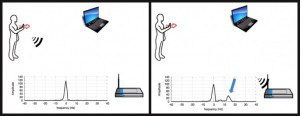
\includegraphics[height=5cm,width=12cm]{2.png}
\counterwithin{figure}{section}
%\counterwithout{figure}{chapter}
\end{figure}

\paragraph{}
 WISEE system use the property of Doppler shift, Doppler shift is the frequency change
of transmitted wave as its source moves relative to the observer. There will be multipath
reflection from the human body, and then human gestures results in pattern of Doppler shift at
the system receiver. So, the movement of user away from the receiver results in negative Doppler
shift, and movement of user towards the receiver results in positive Doppler shift. The challenge
for this system was that result of the human gesture gives very small change in Doppler shifts
that can be very hard to detect from WI-FI transmission. Typically movement around 0.5 m/sec
results in 17 Hz Doppler shift for the 5 GHz WI-FI transmission. For the gesture recognition it is
required to detect the Doppler shifts of few Hertz from 20 MHz WI-FI signals. This solution of
this problem is achieved by transforming the signal which are received from moving object, in to
narrowband pulse with a bandwidth of few Hertz, then system tracks the frequency of this
narrowband pulses to detect the small Doppler shift.

\paragraph{}
In home there may have more than one person who can affects the wireless signals. This
problem is solved by MIMO capability which is inherent to 802.11n, to focus the gesture from a
particular human. The wireless reflection from all the humans can be separated using MIMO
receiver.
\paragraph{}
Finally the experiments were performed for line-of-site, non-line-of-site, and through
wall where the person is in different room from the wireless transmitter and receiver and
achieved results are as follow:
\begin{itemize}
    \item WISEE system can track the 9 human body gesture shown in with 94percent accuracy.
    \item  Using four receiving antenna and one transmitting antenna WISEE can achieve 60%
accuracy.
    \item Using five receiving antenna and single transmitting antenna WISEE can perform the
human gesture classification in presence of other three people who are performing
random gesture.
\end{itemize}

\subsection{Wi-fi signals enable gesture recognition throughout entire home}
\paragraph{}
Forget to turn off the lights before leaving the apartment? No problem. Just raise your
hand, finger-swipe the air, and your lights will power down. Want to change the song playing on
your music system in the other room? Move your hand to the right and flip through the songs.
\paragraph{}
A hand gesture changes the TV channel. A hand gesture changes the TV channel using
WiSee technology. University of Washington computer scientists have developed gesturerecognition
technology that brings this a step closer to reality. Researchers have shown it’s
possible to leverage Wi-Fi signals around us to detect specific movements without needing
sensors on the human body or cameras.
\paragraph{}
By using an adapted Wi-Fi router and a few wireless devices in the living room, users
could control their electronics and household appliances from any room in the home with a
simple gesture.
\paragraph{}
“ This is repurposing wireless signals that already exist in new ways,” said lead researcher
Shyam Gollakota, a UW assistant professor of computer science and engineering. “You can
actually use wireless for gesture recognition without needing to deploy more sensors.”
\paragraph{}
The UW research team that includes Shwetak Patel, an assistant professor of computer
science and engineering and of electrical engineering and his lab, published their findings online
this week. This technology, which they call “WiSee,”


\newpage
\section{RELATED WORK}
\subsection{Wi-Vi Through Radar Wall}
\paragraph{}
Practicing on because through fortify has been done for nearly a decennium. In past time,
inventers are mightily centered on modeling and simulations. Recently few implementations
have been discrimination with humans in moving assertions. This loneliness can be achieved in
tense estate by worn very defective pulsate (about 1 ns) due to which loiter had been improved
between arrival period of reflected eminent off the wall and reflex signal off the pathetic objects
behind defense. Isolation can also be achieved in commonness domain through linear
commonness peep. In this, reflections from appearance at dissimilar position reach with separate
mood. By doing analog filtering of tones corresponds to the wall may be proceed to remove flash
execution. Wi-Vi system has different characteristics as it requires equity bandwidth, and act in
the same range as Wi-Fi. Wi-Vi overcome the requirement for the UWB by worn MIMO nulling
to remove flash effect. These systems unheeded the flash result and tried to work in high
interference caused by the reflections off the wall. They generally think about propagation
caused by moving objects behind the wall. However, the flash result limits their detection
capabilities. Hence, most of those systems square measure incontestable either in simulation or
in free area with no obstruction. Those incontestable with associate obstruction use a lowattenuation
standing wall, and don't work across higher attenuation materials like solid wood or
concrete. Wi-Vi shares the objectives of those devices; but, it introduces a replacement approach
for eliminating the flash result while not broadband transmission. This allows it to figure with
concrete walls and solid wood doors, also as absolutely closed rooms. The sole try that we have a
tendency to square measure alert to that uses Wi-Fi signals so as to check through walls was
created in 2012. This method needed each the transmitter and a reference receiver to be within
the imaged space what is more, the reference receiver within the space has got to be connected to
constant clock because the receiver outside the area. In distinction, Wi-Vi will perform throughwall
imaging while not access to any device on the opposite facet of the wall.

\subsection{Gesture Based Interfaces}
\paragraph{}
In today’s time, industrial gesture recognition systems like the ninteudowii, xbox kinect
etc. These systems won’t to determine a spread of gesture. There are also such system those are
capable of characteristic human gestures by using cameras or putting detector on the anatomy.
Recent work has conjointly mistreatment narrowband signals within the variation of two to four
giga cycle to spot human activities in line of sight by mistreatment microdoppler signatures. Wi-
Vi, however, presents the primary gesture based mostly interface that works in non line of sight
eventualities and even through the wall and thence human isn't need to hold a wireless device or
wear a sensors on their body.
\subsection{Infrared and Thermal Imaging}
\paragraph{}
System supported infrared and thermal imaging extend the human vision on the far side
the visible magnetism vary and permitting U.S.A. to find objects in presence of smoke and
darkness. This technique is operated by capturing infrared or thermal energy mirrored from the
primary obstacle in the line of sight of their sensors. However these technology doesn't enable
U.S.A. to ascertain through walls attributable to having short wavelength (few micro-m to sub mm)
where as Wi-Vi system having varied long wavelength.

\begin{figure}[H]
\centering
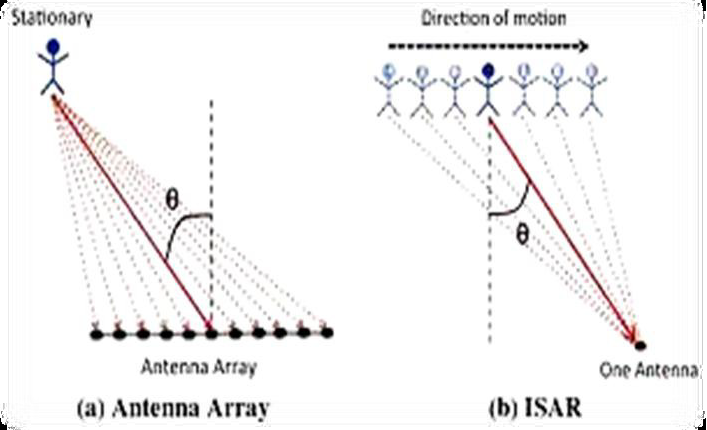
\includegraphics[height=10cm,width=15cm]{4.PNG}
\counterwithin{figure}{section}
%\counterwithout{figure}{chapter}
\end{figure}
\paragraph{}
Above figure shows—A Moving Object as an Antenna Array. In (a), an antenna array is able to locate
an object by steering its beam spatially. In (b), the moving object itself emulates an antenna
array; hence, it acts as an inverse synthetic aperture.

\newpage
\section{TRACKING MOTION}
\subsection{Tracking a single human}
\paragraph{}
Based on the principle of RADAR and SONAR imaging. Wi-Vi is an potentially X-ray
vision created with low power wi-fi signals. This technology uses wi-fi signals to track the
movement of humans behind the walls. RADAR and SONAR works on the doppler effect
.RADAR is an object detective system that uses radio waves to determine range, altitude and
direction or speed of objects. Wi-Vi uses two transmitting antennas and a single receiver. This
two transmitting antennas are low power wi-fi signals. The two antennas transmit identical
signals except that the second antenna is the inverse of first antenna resulting in interference.
Any static objects that the signals hit including the wall create identical reflections these too are
cancelled by this nulling effect. Only those reflections that change between two signals, such as
those from the moving object, arrive back at the receiver. As the person moves from the receiver
his distance changes meaning the time it takes for the reflected signals to make it’s way back to
the receiver changes. The system then uses this information to calculate where the person is at
any one time.

\begin{figure}[H]
\centering
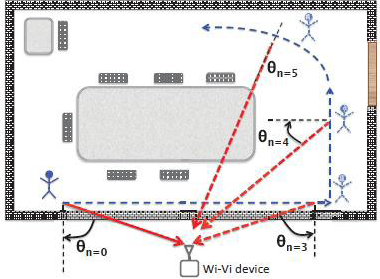
\includegraphics[height=8cm,width=10cm]{5.png}
\counterwithin{figure}{section}
%\counterwithout{figure}{chapter}
\end{figure}

\paragraph{}
In most advanced, through all systems antenna array is employed to trace the human motion.
They steer the arrays beam to see the direction of most energy and this direction corresponds to
the signals abstraction angle of arrival. By following that angle in time, we are able to infer
however the thing moves in area. Most prior through-wall systems track human motion using an
antenna array. They steer the array’s beam to determine the direction of maximum energy. This
direction corresponds to the signal’s spatial angle of arrival. By tracking that angle in time, they
infer how the object moves in space. Wi-Vi, however, avoids using an antenna array for two
reasons: First, in order to obtain a narrow beam and hence achieve a good resolution, one needs a
large antenna array with many antenna elements. This would result in a bulky and expensive
device. Second, since Wi-Vi eliminates the flash effect using MIMO nulling, adding multiple
receive antennas would require nulling the signal at each of them. This would require adding
more transmit antennas, thus making the device even bulkier and more expensive. The figure is
as shown in experimental set up.

\begin{figure}[H]
\centering
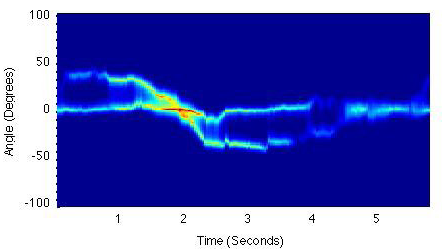
\includegraphics[height=8cm,width=10cm]{6.png}
\counterwithin{figure}{section}
%\counterwithout{figure}{chapter}
\end{figure}

\begin{itemize}
    \item This device can track the human up to range of 8 meters between transmitter and object
with 75percent accuracy and can’t track the human at distance of 9 meters.
    \item  WI-VI can track the moving object up to the 8” thicker concrete wall, 6” thicker hollow
wall and 1.75” solid wooden doors.
    \item As WI-VI replacing the antenna array by ISAR means that the angular resolution in this
system depends on amount of movement. It removes clutter from all static object rather
than just wall.
	\item From the figure it can be concluded, at output we can achieve only magnitude plot
according to the movement of object it doesn’t provide the shape of that object.
\end{itemize}

\subsection{Tracking Multiple Humans}
\paragraph{}
In this section, we show how Wi-Vi extends its tracking procedure to multiple humans.
Our previous discussion about using human motion to emulate an antenna array still holds.
However, each human will emulate a separate antenna array. Since Wi-Vi has a single antenna,
the received signal will be a superposition of the antenna arrays of the moving humans. In
particular, instead of having one curved line as in Figure 3, at any time, there will be as many
curved lines as moving humans at that point in time. However, with multiple humans, the noise
increases significantly. On one hand, each human is not just one object because of different body
parts moving in a loosely coupled way. On the other hand, the signal reflected off all of these
humans is correlated in time, since they all reflect the transmitted signal. The lack of
independence between the reflected signals is important. For example, the reflections of two
humans may combine systematically to dim each other over some period of time.

\begin{figure}[H]
\centering
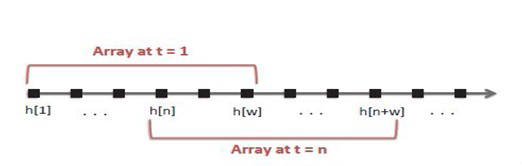
\includegraphics[height=7cm,width=10cm]{7.png}
\counterwithin{figure}{section}
%\counterwithout{figure}{chapter}
\end{figure}


\begin{figure}[H]
\centering
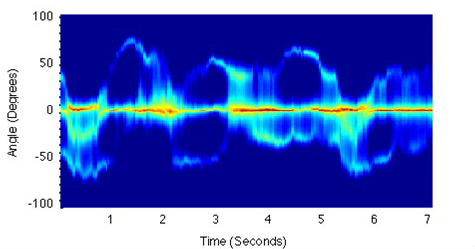
\includegraphics[height=7cm,width=10cm]{8.png}
\counterwithin{figure}{section}
%\counterwithout{figure}{chapter}
\end{figure}
\paragraph{}
Above figure shows Wi-Vi tracking the motion of two humans. The figure shows how the presence
of two humans translates into two curved lines whose angles vary in time, and one straight
line which corresponds to the DC.

\subsection{Eliminating the Flash Effect}
\paragraph{}
Electromagnetic signal produces important attenuation dense obstacles that results in
stronger flash signals than the other mirrored signals off the article. Considering the tables on top
of within which a method rf attenuation of signal is determined through Wi-Fi signal. For
example- once the signal is traveled through interior hollow wall or concrete wall, the Wi-Fi
signal power is reduced by 9dB and 18dB. As mirrored signal on each the reflection constant
likewise because the cross-sectional of object owing to that the particular mirrored signal
becomes weaker .hence, Wi-Vi will increase the sensitivity to the reflection of interest by
victimization the development of interference nulling.
\subsubsection{Nulling to Remove Flash}
\paragraph{}
Recent advances show that MIMO systems can pre-code their transmissions such that the
signal received at a particular antenna is cancelled. Past work on MIMO has used this property to
enable concurrent transmissions and null interference. We observe that the same technique can be
tailored to eliminate the flash effect as well as the direct signal from the transmit to the receive
antenna, thereby enabling Wi-Vi to capture the reflections from objects of interest with minimal
interference.
\paragraph{}
At a high level, Wi-Vi’s nulling procedure can be divided into three phases: initial
nulling, power boosting, and iterative nulling, as shown in Alg. 1. Initial Nulling. In this phase,
Wi-Vi performs standard MIMO nulling. Recall that Wi-Vi has two transmits antennas and one
receive antenna. First, the device transmits a known preamble x only on its first transmit antenna.
This preamble is received at the receive antenna as y= h1x, where h1 is the channel between the
first transmit antenna and the receive antenna. The receiver uses this signal in order to compute
an estimate of the channel h1.
\paragraph{}
Second, the device transmits the same preamble x, this time only on its second antenna, and
uses the received signal to estimate channel h2 between the second transmit antenna and the
receive antenna. Third, Wi-Vi uses these channel estimates to compute the ratio p = = h1/ ˆh2.
Finally, the two transmit antennas transmit concurrently, where the first antenna transmits x and
the second transmits px. Therefore, the perceived channel at the receiver is :-

\begin{figure}[H]
\centering
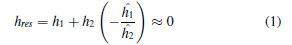
\includegraphics[height=2cm,width=8cm]{8a.png}
\counterwithin{figure}{section}
%\counterwithout{figure}{chapter}
\end{figure}

The algorithm for Wi-Vi nulling is:
\begin{figure}[H]
\centering
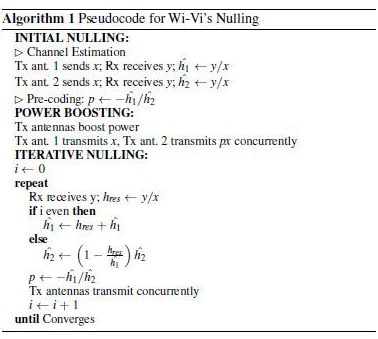
\includegraphics[height=12cm,width=14cm]{9.png}
\counterwithin{figure}{section}
%\counterwithout{figure}{chapter}
\end{figure}

\paragraph{}
In the ideal case, where the estimates h1ˆand ˆ h2 are perfect, the received signal hres
would be equal to zero. Hence, by the end of this phase Wi-Vi has eliminated the signals
reflected off all static objects as well as the direct signal from the transmit antennas to the receive
antenna. If no object moves, the channel will continue being nulled. However, since RF
reflections combine linearly over the medium, if some object moves, its reflections will start
showing up in the channel value.
\paragraph{}
Power Boosting: Simply nulling static reflections, however, is not enough because the signals
due to moving objects behind the wall are too weak. Say, for example, the flash effect was 30 to
40 dB above the power of reflections off moving objects. Even though we removed the flash
effect, we can hardly discern the signal due to moving objects since it will be immersed in the
receiver’s hardware noise. Thus, we next boost the transmitted signal power.5 Note that because
the channel has already been nulled, i.e., hres == 0. this increase in power does not saturate the
receiver’s ADC. However, it increases the overall power that traverses the wall, and, hence,
improves the SNR of the signal due to the objects behind the wall.
\paragraph{}
Iterative Nulling: After boosting the transmit power, residual reflections which were below the
ADC quantization level become measurable. Such reflections from static objects can create
significant clutter in the tracking process if not removed. To address this issue, Wi-Vi performs a
procedure called iterative nulling. At a high level, the objective is simple: we need to null the
signal again after boosting the power to eliminate the residual reflections from static objects. The
challenge, however, is that at this stage, we cannot separately estimate the channels from each of
the two transmit antennas since, after nulling, we only receive a combined channel. We also
cannot remove the nulling and re-estimate the channels, because after boosting the power,
without nulling, the ADC would saturate.

\newpage
\section{TRACKING TECHNIQUES}

\begin{figure}[H]
\centering
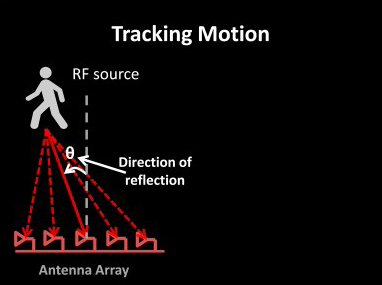
\includegraphics[height=7cm,width=8cm]{10.png}
\counterwithin{figure}{section}
%\counterwithout{figure}{chapter}
\end{figure}

\paragraph{}
The first thing to note is that when the human reflects the signal, it’s as if he is the source
of that signal. We know from wireless textbooks that if you want to track an RF source, you can
do that using an antenna array. By steering the beam of the array, we can find the direction of
from which the signal is coming. Now, when a person moves, that direction would change, and
we are able to track him.

\begin{figure}[H]
\centering
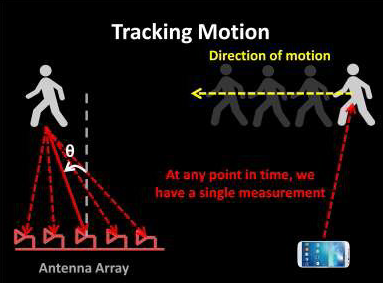
\includegraphics[height=7cm,width=8cm]{11.png}
\counterwithin{figure}{section}
%\counterwithout{figure}{chapter}
\end{figure}

\paragraph{}
Clearly, we cannot build an antenna array on a small device. To address this challenge,
we borrow a technique which has been traditionally used to map different planets from Earth.
The technique uses the movement of the target to emulate an antenna array. So, what do I mean
by that. We have only one receive antenna, which means that at any point in time, we have a
single measurement. Nevertheless, the target is moving.

\begin{figure}[H]
\centering
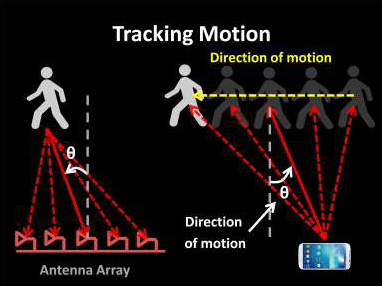
\includegraphics[height=7cm,width=8cm]{12.png}
\counterwithin{figure}{section}
%\counterwithout{figure}{chapter}
\end{figure}

\paragraph{}
This means that at different points in time, he is reflecting the signal from different points
in space.

\paragraph{}
If we consider all of these measurements together, it is as if the person is emulating space
antenna array. Because consecutive measurements in time emulate an antenna array, we can use
standard antenna array beam steering to identify the direction motion of a person.

\begin{figure}[H]
\centering
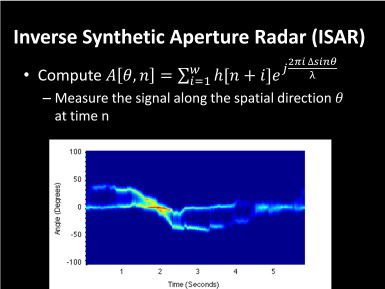
\includegraphics[height=7cm,width=8cm]{12a.png}
\counterwithin{figure}{section}
%\counterwithout{figure}{chapter}
\end{figure}

\paragraph{}
We can use these successive time measurements and apply standard beam forming
equations to obtain the direction of motion.
In fact, what I just described to you is the dual of what Dina described in her talk. Over
there, the receiver had to move to emulate an antenna array, whereas here the movement of the
source naturally emulates the array.

\subsection{Through Wall Gesture-Based Communication.}
\paragraph{}
Wi-Vi has the power during which human WHO doesn't carry any wireless device will
communicate to receiver by exploitation straightforward gestures. Wi-Vi represents these try of
gestures by 0’ bit and 1’ bit. These gestures are later composed by human to make messages that
are having completely different interpretations. In addition, Wi-Vi will develop by exploitation
different existing practices and principles like adding an easy code that may guarantee
dependability, or by reserving an exact pattern of 0’ and 1’s. At this stage this technology
continues to be terribly basic, nevertheless we have a tendency to believe future advancement
scan build it a lot of reliable and communicative.
\subsubsection{Gesture Encoding}
\paragraph{}
At the transmitter side, the ‘0’ and ‘1’ bits must be encoded using some modulation
scheme. Wi-Vi implements this encoding using gesture. One can envision a wide variety of
gestures to represent these bits. However, in choosing our encoding we have imposed three
conditions: 1) the gestures must be composable – i.e. at the end of each bit, whether ‘0’ or ‘1’,
the human should be back in the same initial state as the start of the gesture.
\paragraph{}
This enables the person to compose multiple such gestures to send a longer message. 2)
The gestures must be simple so that a human finds it easy to perform them and compose them. 3)
The gestures should be easy to detect and decode without requiring sophisticated decoders, such
as machine learning classifiers.

\begin{figure}[H]
\centering
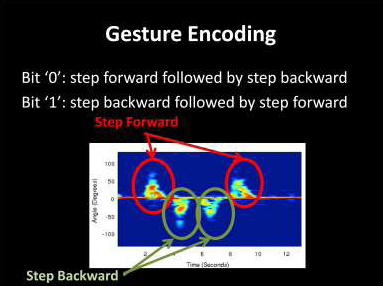
\includegraphics[height=7cm,width=8cm]{13.png}
\counterwithin{figure}{section}
%\counterwithout{figure}{chapter}
\end{figure}

\paragraph{}
Given the above constraints, we have selected the following gestures to modulate the bits:
a ‘0’ bit is a step forward followed by a step backward; a ‘1’ bit is a step backward followed by a
step forward. This modulation is similar to Manchester encoding, where a ‘0’ bit is represented
by a falling edge of the clock, (i.e., an increase in the signal value followed by a decrease,) and a
‘1’ bit is represented by a rising edge of the clock, (i.e., a reduction in signal value followed by
an increase).
\paragraph{}
Figure shows the signal captured by Wi-Vi, at the output of the smoothed MUSIC
algorithm for each of these two gestures. Taking a step forward towards the Wi-Vi device
produces a positive angle, whereas taking a step backward produces a negative angle. The exact
values of the produced angles depend on whether the human is exactly oriented towards the
device. Recall that the angle is between the vector orthogonal to the motion and the line
connecting the human to the Wi-Vi device, and its sign is positive when the human is moving
toward Wi-Vi and negative when the human moves away from Wi-Vi.

\subsubsection{Gesture Decoding}
\paragraph{}
Decoding the above gestures is fairly simple and follows standard communication
techniques. Specifically, Wi-Vi’s decoder takes as input A![!, n]. Similar to a standard decoder
[16], Wi-Vi applies a matched filter on this signal. However, since each bit is a combination of
two steps, forward and backward, Wi-Vi applies two matched filters: one for the step forward
and one for the step backward. Because of the structure of the signal shown in Figure 4, the two
matched filters are simply a triangle above the zero line, and an inverted triangle below the zero
line. Wi-Vi applies these filters separately on the received signal, then adds up their output.

\begin{figure}[H]
\centering
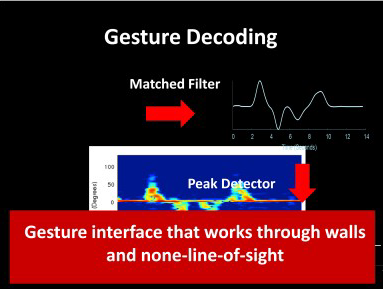
\includegraphics[height=7cm,width=8cm]{14.png}
\counterwithin{figure}{section}
%\counterwithout{figure}{chapter}
\end{figure}

\paragraph{}
So, for example, a positive peak followed by a negative peak represents bit 0 and a
negative peak followed by a positive peak represents a bit 1. This is just like manchester coding.
With this capability, Wi-Vi enables a new gesture-based interface that works through walls and in
NLOS. Hence, you are not limited you to stand in front of your game console. You can move
freely and be even in a different room and still interact with your game.

\newpage
\section{ADVANTAGES AND LIMITATIONS}
\subsection{Advantages:}

\begin{itemize}
    \item Wi-Vi is relatively a low-power, low-cost, low-bandwidth, and accessible to average
users.
	\item Wi-Vi requires only few MHz of bandwidth and operates in the same range as Wi-Fi. It
operates in ISM band.
	\item Wi-Vi can perform through-wall imaging without access to any device the other side of
the wall.
	\item Wi-Vi employs signals whose wavelengths are 12.5 cm.
	\item Extend human vision beyond the visible electromagnetic range, allowing us to detect
objects in the dark or in smoke.
\end{itemize}

\subsection{Limitations:}

\begin{itemize}
    	\item Display has very low resolution.
	\item We cannot detect humans behind concrete walls thicker than 8.
	\item To achieve a narrow beam the human needs to move by about 4 wavelengths (i.e., about
50 cm).
\end{itemize}

\newpage
\section{CONCLUSION AND FUTURE ENHANCEMENT}
\paragraph{}
Wi-Vi is a wireless technology that uses Wi-Fi signals to find moving humans
behind walls and in closed rooms. In distinction to previous systems, that square measure
targeted for the military, Wi-Vi allows tiny low cost see- through-wall devices that operate within
the philosophy band, rendering them possible to the final public.
\paragraph{}
Wi-Vi additionally establishes a channel between itself and a person's behind a wall,
permitting him/her to speak directly with Wi-Vi while not carrying any sending device. we tend
to believe that Wi-Vi is associate degree instance of a broader set of practicality that future
wireless networks can offer. Future Wi-Fi networks can probably expand on the far side
communications and deliver services like indoor localization, sensing, and management. Wi-Vi
demonstrates a sophisticated variety of Wi-Fi-based sensing and localization by victimization
Wi-Fi to trace humans behind wall, even after they don't carry a wireless device. It additionally
raises problems with importance to the networking community pertinent to user privacy and laws
regarding the utilization of Wi-Fi signals. Finally, Wi-Vi bridges progressive networking
techniques with human-computer interaction. It motivates a replacement variety of user
interfaces that swear entirely on victimization the reflections of a transmitted RF signal to spot
human gestures. We tend to envision that by investing finer nulling techniques and using higher
hardware, the system will evolve to seeing humans through denser artifact and with a extended
vary. These enhancements can additional permit Wi-Vi to capture higher quality pictures
enabling the gesture-based interface to become additional communicative hence promising new
directions for computer game.

\paragraph{}
\textbf{FUTURE ENHANCEMENT:}
\begin{itemize}
	\item Wi-vi could be built into a smartphone or a special handheld device.
	\item High quality images
	\item Evolution of seeing humans through denser building material and with a longer range.
\end{itemize}

\newpage
\cleardoublepage
\section{REFERENCES}
\begin{thebibliography}{9}


\bibitem{d} V. Mura, L. Ghiani, G. L. Marcialis, F. Roli, D. A. Yambay, and
S. A. Schuckers,\emph{ “Livdet 2015 fingerprint liveness detection competition
2015.”}
\bibitem{d} J. Galbally, F. Alonso-Fernandez, J. Fierrez, and J. Ortega-Garcia,\emph{ “A
high performance fingerprint liveness detection method based on quality
related features,” }Future Generation Computer Systems, vol. 28, no. 1,
pp. 311–321, 2012.
\bibitem{d} Y. Chen, A. Jain, and S. Dass, \emph{“Fingerprint deformation for spoof
detection,” }in Biometric Symposium, 2005, p. 21.
\bibitem{d} B. Tan and S. Schuckers,\emph{ “Comparison of ridge-and intensity-based
perspiration liveness detection methods in fingerprint scanners,”} in
Defense and Security Symposium. International Society for Optics and
Photonics, 2006, pp. 62 020A–62 020A.
\bibitem{d} P. Coli, G. L. Marcialis, and F. Roli, \emph{“Fingerprint silicon replicas: static
and dynamic features for vitality detection using an optical capture
device,”} International Journal of Image and Graphics, vol. 8, no. 04,
pp. 495–512, 2008.
\bibitem{d} P. D. Lapsley, J. A. Lee, D. F. Pare Jr, and N. Hoffman, \emph{“Anti-fraud
biometric scanner that accurately detects blood flow,”} Apr. 7 1998, uS
Patent 5,737,439.
\bibitem{d}A. Antonelli, R. Cappelli, D. Maio, and D. Maltoni, \emph{“Fake finger detection
by skin distortion analysis,” }Information Forensics and Security,
IEEE Transactions on, vol. 1, no. 3, pp. 360–373, 2006.
\bibitem{d} Baldisserra, A. Franco, D. Maio, and D. Maltoni, \emph{“Fake fingerprint
detection by odor analysis,”} in Advances in Biometrics. Springer, 2005,
pp. 265–272.
\bibitem{d} A. K. Jain, Y. Chen, and M. Demirkus,\emph{ “Pores and ridges: Highresolution
fingerprint matching using level 3 features,”} Pattern Analysis
and Machine Intelligence, IEEE Transactions on, vol. 29, no. 1, pp.
15–27, 2007.

\bibitem{d}Purneet Kaur , Jaspreet Kaur {"Fingerprint Recognition Using Genetic Algorithm and Neural Network"} 
\bibitem{d}Aliyu Tukur {"Fingerprint Recognition and Matching" }

\bibitem{d}  Adrian Lim Hooi Jinl, Ai Chekima, Jamal Ahmad Dargham, and Liau Chung Fan {"Fingerprint identification and recognition using backpropagation neural network"}
\bibitem{d}Han-Ul Jang, Hak-Yeol Choi, Dongkyu Kim, Jeongho Son,and Heung-Kyu Lee {"Fingerprint Spoof Detection Using Contrast
Enhancement and Convolutional
Neural Networks"}

\bibitem{d}Diego Gragnaniello, Giovanni Poggi, Carlo Sansone and Luisa Verdoliva {"Fingerprint Liveness Detection
based on Weber Local Image Descriptor"}


\bibitem Tarang Chugh, Kai Cao, and Anil K. Jain, {"Fingerprint Spoof Buster"}


\bibitem Ravi Subban and Dattatreya P. Mankame
{"A Study of Biometric Approach Using Fingerprint
Recognition"} 

\bibitem W. F. Leung, S. H. Leung, W. H. Lau and Andrew Luk  {"Fingerprint recognition using neural network"}
\bibitem
Hriday Goyal, Gaurav Verma, Chetan Arora, { "Fingerprint Detection and Authentication using feature extraction based on Minutiae" }

\bibitem  Qiaoqiao Li,Patrick P. K. Chan, {"Fingerprint liveness detection based on binarized statistical image feature with sampling from Gaussian distribution"}

\bibitem{site1}https://ieeexplore.ieee.org/document/7390065/(Accessed On 18/03/18)



\end{thebibliography}


\end{document}